\documentclass[11pt, a4paper]{article}

\usepackage[utf8]{inputenc}
\usepackage[T1]{fontenc}
\usepackage{amsmath, amssymb}
\usepackage{graphicx}
\usepackage{booktabs}
\usepackage{geometry}
\geometry{margin=1in}
\usepackage{natbib}
\usepackage{xcolor}
\usepackage[colorlinks=true, allcolors=blue!55!black]{hyperref}

% All quantities come from numbers.tex, generated by code/make_numbers.py from
% the released data. No figure in this manuscript is typed by hand.
% Generated by code/make_numbers.py. Do not edit by hand.
% Every quantity quoted in the manuscript is defined here.

\newcommand{\Nrefs}{22{,}479}
\newcommand{\Npapers}{919}
\newcommand{\Nrefsperpaper}{24.5}
\newcommand{\Ntruncated}{171}
\newcommand{\Nflag}{307}
\newcommand{\Nverified}{22{,}172}
\newcommand{\Flagrate}{1.37}
\newcommand{\NrefsSixteen}{8{,}905}
\newcommand{\NpapersSixteen}{383}
\newcommand{\NflagSixteen}{80}
\newcommand{\FlagrateSixteen}{0.898}
\newcommand{\NrefsTwentythree}{7{,}620}
\newcommand{\NpapersTwentythree}{289}
\newcommand{\NflagTwentythree}{101}
\newcommand{\FlagrateTwentythree}{1.325}
\newcommand{\NrefsTwentyfive}{3{,}541}
\newcommand{\NpapersTwentyfive}{136}
\newcommand{\NflagTwentyfive}{86}
\newcommand{\FlagrateTwentyfive}{2.429}
\newcommand{\NrefsTwentysix}{2{,}413}
\newcommand{\NpapersTwentysix}{111}
\newcommand{\NflagTwentysix}{40}
\newcommand{\FlagrateTwentysix}{1.658}
\newcommand{\NrefsQbioSixteen}{2{,}658}
\newcommand{\NpapersQbioSixteen}{95}
\newcommand{\NflagQbioSixteen}{15}
\newcommand{\FlagrateQbioSixteen}{0.564}
\newcommand{\NrefsQbioTwentythree}{2{,}398}
\newcommand{\NpapersQbioTwentythree}{91}
\newcommand{\NflagQbioTwentythree}{16}
\newcommand{\FlagrateQbioTwentythree}{0.667}
\newcommand{\NrefsCsSixteen}{2{,}963}
\newcommand{\NpapersCsSixteen}{140}
\newcommand{\NflagCsSixteen}{11}
\newcommand{\FlagrateCsSixteen}{0.371}
\newcommand{\NrefsCsTwentythree}{2{,}868}
\newcommand{\NpapersCsTwentythree}{128}
\newcommand{\NflagCsTwentythree}{32}
\newcommand{\FlagrateCsTwentythree}{1.116}
\newcommand{\NrefsCsTwentyfive}{2{,}938}
\newcommand{\NpapersCsTwentyfive}{123}
\newcommand{\NflagCsTwentyfive}{85}
\newcommand{\FlagrateCsTwentyfive}{2.893}
\newcommand{\NrefsNipsSixteen}{3{,}284}
\newcommand{\NpapersNipsSixteen}{148}
\newcommand{\NflagNipsSixteen}{54}
\newcommand{\FlagrateNipsSixteen}{1.644}
\newcommand{\NrefsNipsTwentythree}{2{,}354}
\newcommand{\NpapersNipsTwentythree}{70}
\newcommand{\NflagNipsTwentythree}{53}
\newcommand{\FlagrateNipsTwentythree}{2.251}
\newcommand{\NrefsNipsTwentyfive}{603}
\newcommand{\NpapersNipsTwentyfive}{13}
\newcommand{\NflagNipsTwentyfive}{1}
\newcommand{\FlagrateNipsTwentyfive}{0.166}
\newcommand{\NrefsGenTwentysix}{2{,}413}
\newcommand{\NpapersGenTwentysix}{111}
\newcommand{\NflagGenTwentysix}{40}
\newcommand{\FlagrateGenTwentysix}{1.658}
\newcommand{\Nmatchcorrect}{13{,}195}
\newcommand{\Nmatchweak}{3{,}357}
\newcommand{\Nmatchwrong}{5{,}620}
\newcommand{\Pcmatchcorrect}{59.51}
\newcommand{\Pcmatchweak}{15.14}
\newcommand{\Pcmatchwrong}{25.35}
\newcommand{\Pcmatchcorrectmin}{50.3}
\newcommand{\Pcmatchcorrectmax}{79.8}
\newcommand{\Matchcorrectminvenue}{NeurIPS 2025}
\newcommand{\Matchcorrectmaxvenue}{Arxiv Bio 2023}
\newcommand{\StageAn}{307}
\newcommand{\StageArecovered}{197}
\newcommand{\StageAfuzzy}{64}
\newcommand{\StageAunresolved}{46}
\newcommand{\PcStageArecovered}{64.2}
\newcommand{\PcStageAfuzzy}{20.8}
\newcommand{\PcStageAunresolved}{15.0}
\newcommand{\StageAcomplete}{yes}
\newcommand{\Cohorttrendchisq}{45.19}
\newcommand{\Cohorttrenddf}{2}
\newcommand{\Cohorttrendp}{p = 1.5 \times 10^{-10}}
\newcommand{\Cstrendchisq}{68.73}
\newcommand{\Cstrenddf}{2}
\newcommand{\Cstrendp}{p < 10^{-14}}
\newcommand{\Qbiop}{p = 0.72}
\newcommand{\Nipsp}{p = 0.11}
\newcommand{\StageBn}{46}
\newcommand{\StageBseg}{21}
\newcommand{\PcStageBseg}{45.7}
\newcommand{\StageBnotref}{17}
\newcommand{\PcStageBnotref}{37.0}
\newcommand{\StageBrule}{5}
\newcommand{\PcStageBrule}{10.9}
\newcommand{\StageBcov}{3}
\newcommand{\PcStageBcov}{6.5}
\newcommand{\StageBfab}{0}
\newcommand{\PcStageBfab}{0.0}
\newcommand{\StageBastro}{18}
\newcommand{\StageBcomplete}{yes}
\newcommand{\StageCn}{200}
\newcommand{\StageCconfirmed}{125}
\newcommand{\StageCfuzzy}{58}
\newcommand{\StageCunresolved}{17}
\newcommand{\PcStageCconfirmed}{62.5}
\newcommand{\PcStageCfuzzy}{29.0}
\newcommand{\PcStageCunresolved}{8.5}
\newcommand{\StageCcomplete}{yes}
\newcommand{\StageCrule}{10}
\newcommand{\StageCcov}{4}
\newcommand{\StageCnotref}{1}
\newcommand{\StageCunconf}{2}
\newcommand{\StageCfab}{0}
\newcommand{\Boundfab}{1.49}
\newcommand{\Boundconservative}{3.11}
\newcommand{\LigQbioSixteen}{14.18}
\newcommand{\GlueQbioSixteen}{4.40}
\newcommand{\LigQbioTwentythree}{7.67}
\newcommand{\GlueQbioTwentythree}{6.51}
\newcommand{\LigCsSixteen}{22.04}
\newcommand{\GlueCsSixteen}{2.94}
\newcommand{\LigCsTwentythree}{2.09}
\newcommand{\GlueCsTwentythree}{5.58}
\newcommand{\LigCsTwentyfive}{0.82}
\newcommand{\GlueCsTwentyfive}{5.07}
\newcommand{\LigNipsSixteen}{16.50}
\newcommand{\GlueNipsSixteen}{2.04}
\newcommand{\LigNipsTwentythree}{5.27}
\newcommand{\GlueNipsTwentythree}{2.80}
\newcommand{\LigNipsTwentyfive}{7.30}
\newcommand{\GlueNipsTwentyfive}{4.64}
\newcommand{\LigGenTwentysix}{0.21}
\newcommand{\GlueGenTwentysix}{4.81}
\newcommand{\Damagerr}{1.55}
\newcommand{\RhoLig}{-0.617}
\newcommand{\RhoGlue}{+0.017}
\newcommand{\RhoDamage}{-0.283}
\newcommand{\Preprintrr}{1.78}
\newcommand{\NonpreprintrateCsSixteen}{0.36}
\newcommand{\PreprintshareCsSixteen}{6.4}
\newcommand{\NonpreprintrateCsTwentythree}{1.06}
\newcommand{\PreprintshareCsTwentythree}{20.9}
\newcommand{\NonpreprintrateCsTwentyfive}{2.56}
\newcommand{\PreprintshareCsTwentyfive}{24.3}
\newcommand{\Nbench}{400}
\newcommand{\Nbenchgroup}{100}
\newcommand{\Naiveprec}{58.33}
\newcommand{\Naiverec}{63.00}
\newcommand{\Naivefone}{60.58}
\newcommand{\Naivefprintact}{42.0}
\newcommand{\Naivefprstressed}{48.0}
\newcommand{\Cieprec}{66.84}
\newcommand{\Cierec}{65.50}
\newcommand{\Ciefone}{66.16}
\newcommand{\Ciefprintact}{15.0}
\newcommand{\Ciefprstressed}{50.0}


% Anything not yet established by the audit is marked with this command, which
% is deliberately conspicuous so that no unfilled quantity can reach a
% submission. code/check_manuscript.py refuses to pass while one survives.
\newcommand{\pending}[1]{\textcolor{red}{\textbf{[PENDING: #1]}}}

\title{Neither Flag nor Pass: Measurement Error in Automated Reference Verification}

\author{
    Diletta Abbonato\textsuperscript{1,*} \\
    \small \textsuperscript{1}CPS Department, University of Turin, Turin, Italy \\
    \small \textsuperscript{*}Corresponding author: \texttt{diletta.abbonato@unito.it}
}
\date{}

\begin{document}

\maketitle

\begin{abstract}
\noindent Automated reference screening has become an operational stage of scientific publishing, and the counts it produces are increasingly read as evidence about citation integrity. Those counts rest on a matching step whose error properties have received little attention. This paper introduces \textit{CheckIfExist}, an open-source and fully deterministic verification framework that normalizes extracted reference strings, queries five bibliographic sources in parallel and applies an explicit agreement rule on title, authors and year, and uses it to examine the error properties of the screening step itself. The empirical basis is a corpus of \Nrefs{} reference strings extracted from \Npapers{} arXiv preprints and NeurIPS proceedings papers published between 2016 and 2026 and screened by a single-source matcher of the kind commonly deployed. Two results follow, and they point in opposite directions. Of the \Nflag{} strings the matcher leaves unresolved, normalization and multi-source retrieval recover \PcStageArecovered{}\% outright and leave only \PcStageAunresolved{}\% genuinely unmatched, so the unresolved class is dominated by recoverable retrieval failures rather than by absent works. Less expectedly, the accepted class is also unreliable: applying the agreement rule to the record the matcher actually retrieved shows that only \Pcmatchcorrect{}\% of the \Nverified{} accepted references correspond to the work cited, while \Pcmatchwrong{}\% resolve to a different publication. Individual resolution of every string that survives both checks locates no fabricated reference, and bounds fabrication prevalence in the accepted stratum at \Boundfab{}\% under the most favourable reading and \Boundconservative{}\% under the most adverse. Both error rates vary across venues and years in ways that a common trend in authorship does not readily explain, and two candidate mechanisms, extraction damage and a compositional shift towards preprints, are tested and fail. We would maintain that an unverifiable-citation rate computed from a permissive single-source matcher measures the instrument at least as much as it measures the literature. The tool, the corpus and the analysis code are released openly.

\vspace{6pt}
\noindent \textbf{Keywords:} Scientometrics; Bibliographic verification; Citation quality; Research integrity; Large language models; Scholarly databases.
\end{abstract}

\section{Introduction}
\label{sec:intro}

Bibliographic references are part of the infrastructure of scientific communication. They assign credit, allow readers to retrace an argument, and supply the raw material for the citation indicators used in research assessment. Errors in reference metadata therefore do not stay inside the manuscript in which they occur, but propagate into retrieval, indexing and evaluation.

The diffusion of large language models has given this old problem a new urgency. Experimental work has repeatedly shown that language models fabricate bibliographic references under a wide range of prompting conditions \citep{bhattacharyya2023, walters2023, day2023, eysenbach2023}, and recent studies document such references in the published record itself. \citet{sakai2026} examined the full recent proceedings of the major computational linguistics conferences and found a substantial and sharply growing share of papers carrying hallucinated citations, with the increase concentrated in the most recent year observed. \citet{zhao2026} scaled the exercise to the reference lists of several large repositories, and report the highest rates in the social sciences and in computer science \citep{naturesocsci2026}. \citet{russinovich2026} adopt a deliberately strict definition, restricted to non-existent works and substantial author-list mismatches, and nonetheless find that a far from negligible share of recent papers at leading machine learning and security venues carries them. Publishers and repositories have responded, and arXiv now suspends authors who submit unchecked machine-generated references \citep{naturebanned2026, naturepolluting2026}.

These studies share an underlying operation. A reference string is extracted from a manuscript, matched against one or more bibliographic databases, and either resolved or flagged. The rates that follow are then reported as rates of hallucinated, fabricated or invalid citations. Given that such rates now inform desk rejections and submission bans, it seems reasonable to ask what the matching step actually measures, and the question has received comparatively little attention.

There are good reasons, familiar to this journal, to expect the answer to be complicated. Bibliographic databases differ substantially in what they index, and monographs, dissertations, technical reports and non-English literature remain only partly covered \citep{martinmartin2018, visser2021, verabaceta2019, priem2022}. It follows that the absence of a match in any single database is weak evidence that a cited work does not exist, and yet screening systems in operational use are frequently built on exactly one source. Extraction corrupts strings before any database is queried, since the text layer of a PDF depends on the typesetting engine that produced it and reference parsers are known to be sensitive to document quality and formatting convention \citep{lopez2009, tkaczyk2015}. An unresolved query therefore conflates coverage, extraction fidelity, parser behaviour and, possibly, fabrication. This much has been acknowledged in passing by several of the studies cited above. What has not been examined, to our knowledge, is the converse: whether a resolved query establishes that the cited work exists.

Existing verification tools are oriented towards the first question. They are evaluated on their ability to detect invalid references, and report their performance in terms of the fabrications found. The complementary quantities, namely the false alarms generated by extraction artifacts and coverage gaps, and the false confirmations generated by permissive matching, are seldom reported. That asymmetry is defensible when the output feeds a retrospective study. It is harder to defend once the same output informs an editorial decision about an individual manuscript. It is worth noting that the architecture described by \citet{russinovich2026}, which resolves entries against multiple sources and escalates the unresolved residual to web search, is precisely a response to the first problem, which suggests some convergence on multi-source retrieval with escalation as the sensible design.

This paper makes two contributions. The first is \textit{CheckIfExist}, an open-source verification framework that is deterministic by construction, queries several complementary bibliographic sources in parallel, and applies an explicit and auditable agreement rule rather than model-based inference. Section~\ref{sec:tool} describes it. The second is an application of that framework to the measurement problem, on a corpus of reference strings drawn from arXiv preprints and NeurIPS proceedings papers, spanning a pre-LLM baseline and a sequence of later cohorts. We screen the corpus with a single-source matcher of the kind commonly deployed, and then examine both of its output classes: for the unresolved class we apply normalization and multi-source retrieval and record what is recovered, and for the accepted class we apply the agreement rule to the record the matcher itself retrieved and record how often that record is the work cited. Both classes turn out to be unreliable, in opposite directions, and the failures resolve on inspection into limitations of coverage, of extraction and of the matching rule rather than into absent works. Both error rates also vary systematically across venues and years.

\section{The CheckIfExist framework}
\label{sec:tool}

CheckIfExist is deterministic by design. Given the same input it returns the same output, and every classification can be reproduced independently from the released code. No model-based inference is used at any stage. This is a deliberate choice rather than a limitation of implementation. Where an automated assessment may lead to a desk rejection or a submission ban, an auditable rule that a referee or an author can inspect seems preferable to a score that cannot be interrogated, and reproducibility is in any case a precondition for using such output in bibliometric work.

Let $R$ denote a raw reference string. Normalization $\Phi(R)$ resolves typographic ligatures into their constituent characters, applies Unicode compatibility decomposition, strips combining marks, and separates bibliographic fields that PDF extraction frequently concatenates, such as merged author and year blocks. Each candidate record retrieved from a source is represented as a tuple $M = (T_M, A_M, Y_M)$ of title, author surnames and publication year. Title agreement combines a character-level and a token-level component, since bibliographic styles differ in punctuation, capitalization and word order:
\begin{equation}
S_{\mathrm{Title}} = \max \left( S_{\mathrm{Lev}}\big(\Phi(R), T_M\big),\;
\frac{|\tau(\Phi(R)) \cap \tau(T_M)|}{|\tau(T_M)|} \right),
\end{equation}
where $S_{\mathrm{Lev}}$ is the normalized Levenshtein similarity and $\tau(s)$ the set of alphanumeric tokens of length at least three. Author agreement is the share of the candidate's surnames present in the normalized string, which is more robust than a symmetric coefficient given that author lists are frequently truncated during extraction:
\begin{equation}
A_{\mathrm{Hit}} = \frac{\left| \{a \in A_M : a \subseteq \Phi(R)\} \right|}{|A_M|}.
\end{equation}
Publication year is treated as a tolerance rather than an exact match, $B_{\mathrm{Year}} = \mathbb{I}(|Y_R - Y_M| \le 1)$, which accommodates early online publication, proceedings versions and indexing delay. A reference is classified as verified when some source returns a record satisfying $S_{\mathrm{Title}} \ge 0.85$, $A_{\mathrm{Hit}} \ge 0.50$ and $B_{\mathrm{Year}}$ not violated; as fuzzy when title agreement falls between 0.50 and 0.85; and as unresolved otherwise. Thresholds prioritise precision over recall, on the reasoning that an unresolved classification is a routing decision that sends a string for inspection rather than a verdict on the reference.

The rule is evaluated across five sources queried in parallel, namely Crossref, OpenAlex \citep{priem2022}, Semantic Scholar, arXiv and DBLP, and a reference is verified if any of them satisfies it. The rationale is the coverage literature cited above: a work absent from one index is frequently present in another, and the five differ systematically in the segments of the record they cover.

Two implementation points should be recorded, since both bear on how the results below are to be read. The first concerns normalization. The function $\Phi$ described above is the one implemented in the released analysis code and applied throughout Section~\ref{sec:results}; the public dashboard currently applies a narrower normalization that decomposes accented characters but leaves typographic ligatures intact, so it does not at present recover the ligature artifacts discussed below. Aligning the two is straightforward and is the obvious next revision of the tool, but we would rather state the difference than let a reader assume the deployed artifact and the evaluated procedure are identical. The second is easy to get wrong and was got wrong here. OpenAlex and arXiv do not respond usefully to a full punctuated reference string submitted as a query, and return nothing under those conditions. A first version of the analysis reported below queried them that way and was in effect running on Crossref alone while reporting five sources. Testing the two query forms on five references known to be genuine returned zero hits for the full-string form and five for a keyword form, and correcting this moved the residual reported in Section~\ref{sec:results} from 60 strings to \StageAunresolved{}.

The framework is distributed as an open-source web application requiring no installation or account.\footnote{Dashboard: \url{https://zabbonat.github.io/References-Validation/}. Source: \url{https://github.com/zabbonat/References-Validation}.} It accepts a single reference, a pasted bibliography, a BibTeX file, or a PDF or DOCX manuscript, in which case it locates the bibliography and segments it before verification. Beyond the verification verdict it validates DOIs against the resolved record, flags retractions through Crossref and OpenAlex metadata, and returns corrected records built from the retrieved metadata rather than from the input, exportable as BibTeX, RIS, APA, MLA, ISO 690 or a spreadsheet report. A predatory-venue check is also present but rests on a short illustrative list and is not evaluated here.

Table~\ref{tab:benchmark} reports an evaluation on a constructed pool of \Nbench{} cases in four equal groups of \Nbenchgroup{}. Two groups are negatives that a verification system should not flag, namely intact references that resolve across sources and genuine references corrupted by typographic artifacts of the kind extraction introduces. Two are positives that it should flag, namely fabricated citations taken from published studies of model-generated references \citep{bhattacharyya2023, walters2023} and near-misses pairing genuine titles with incorrect author lists. Including stressed negatives is the point of the design, since a pool composed only of fabrications cannot measure false-alarm behaviour at all.

\begin{table}[htbp]
\centering
\caption{Evaluation on the constructed pool of \Nbench{} cases. False-positive rates are reported separately for intact and stressed negatives ($n = \Nbenchgroup{}$ each).}
\label{tab:benchmark}
\vspace{4pt}
\begin{tabular}{lrrrrr}
\toprule
\textbf{Pipeline} & \textbf{Precision} & \textbf{Recall} & \textbf{F1} & \textbf{FPR intact} & \textbf{FPR stressed} \\
\midrule
Single-source pass    & \Naiveprec{}\% & \Naiverec{}\% & \Naivefone{}\% & \Naivefprintact{}\% & \Naivefprstressed{}\% \\
\textit{CheckIfExist} & \Cieprec{}\%   & \Cierec{}\%   & \Ciefone{}\%   & \Ciefprintact{}\%   & \Ciefprstressed{}\% \\
\bottomrule
\end{tabular}
\end{table}

On intact genuine references, which can fail only because a source does not index them, multi-source matching lowers the false-alarm rate from \Naivefprintact{}\% to \Ciefprintact{}\%, at comparable recall. On stressed negatives the two are indistinguishable, at \Naivefprstressed{}\% and \Ciefprstressed{}\%, so normalization does not recover the corrupted strings in that group. The explanation appears to lie with the corruption generator rather than with normalization, since it applies distortions harsher than those observed in the corpus and corruptions that perturb the token content of a title defeat both components of $S_{\mathrm{Title}}$. We would therefore read the stressed group as a relative comparison under controlled stress and not as an estimate of deployment behaviour. Three further caveats belong here rather than in a footnote. Absolute discrimination is modest for both pipelines, with F1 close to two thirds, which is a further reason to treat a flag as a routing decision. The decision thresholds were calibrated on the same pool used for this evaluation, so the figures may carry an optimistic bias. And the comparison pipeline is a deliberately simple implementation rather than a deployed screener, so Table~\ref{tab:benchmark} establishes the direction of the difference and not its magnitude in production.

\section{Data and methods}
\label{sec:data}

The corpus consists of \Nrefs{} reference strings drawn from the bibliographies of \Npapers{} papers, distributed across nine venue-year strata and grouped into four temporal cohorts. The 2016 cohort provides a pre-LLM baseline, the 2023 cohort covers the early post-ChatGPT period, the 2025 cohort represents an environment in which model-assisted writing is widespread, and a 2026 cohort samples recent general arXiv submissions. Composition varies by design: the 2016 and 2023 cohorts combine arXiv \textit{cs.AI}, arXiv \textit{q-bio} and NeurIPS, the 2025 cohort combines \textit{cs.AI} and NeurIPS, and the 2026 cohort consists of general arXiv submissions. Cohort sizes are \NpapersSixteen{}, \NpapersTwentythree{}, \NpapersTwentyfive{} and \NpapersTwentysix{} papers, yielding an average of \Nrefsperpaper{} references per paper. The heterogeneity across cohorts both permits and complicates the temporal comparison, and Section~\ref{sec:mechanisms} addresses the confound directly.

References were extracted from the compiled PDF files using PyMuPDF, version 1.27.2. For each document the text layer of the final ten pages was retrieved, the bibliography located by matching a set of section-heading patterns, and the block segmented into individual strings on enumeration markers. Segments shorter than fifteen characters were discarded and at most fifty references per paper were retained, a cap that truncates the bibliography of \Ntruncated{} of the \Npapers{} papers. Three features of this design condition what follows. Extraction operates on the compiled PDF and not on the source, so the text layer written by the typesetting engine forms part of the measurement instrument. The segmentation is heuristic rather than model-based, which keeps it transparent but admits some non-reference material into the corpus. And no manual correction was applied before verification, so the corpus reflects what an automated screening system would actually receive. We regard the second feature as a limitation and the first and third as necessary if the exercise is to be informative about deployed systems.

Each extracted string was then screened by a single-source matcher, which submits the string as a bibliographic query to Crossref, falls back to Semantic Scholar when Crossref returns nothing, and accepts the first record returned. A string for which no record is returned is recorded as unresolved. This procedure is deliberately simple and close to what a minimal screening implementation does. Accepting the top-ranked record without further comparison is a common shortcut, and the consequences of that shortcut are one of the two results reported below.

Three analyses follow, and they differ in what they require. The first re-verifies every unresolved string by applying $\Phi$ and querying four sources under the agreement rule of Section~\ref{sec:tool}; Semantic Scholar is excluded here because it rate-limits unauthenticated bulk querying. This is fully deterministic and its evidence is a DOI or repository identifier. The second applies the same agreement rule retrospectively to the record the screening pass itself accepted, which requires no further retrieval because that record was stored, and therefore covers the entire accepted stratum rather than a sample. The third measures, across the nine strata, the prevalence of extraction damage and of citations to material that Crossref indexes poorly, in order to test two candidate explanations of the temporal pattern.

\section{Results}
\label{sec:results}

\subsection{The unresolved class}
\label{sec:unresolved}

The single-source pass leaves \Nflag{} of the \Nrefs{} strings unresolved, an overall rate of \Flagrate{}\%. Table~\ref{tab:venue} reports the distribution across strata and Figure~\ref{fig:unresolved} displays it. Read at face value the series is consistent with the narrative motivating much of the recent literature, since the cohort rate rises from \FlagrateSixteen{}\% in 2016 to \FlagrateTwentythree{}\% in 2023 and \FlagrateTwentyfive{}\% in 2025, an increase unlikely to be chance ($\chi^2 = \Cohorttrendchisq{}$, $\mathrm{df} = \Cohorttrenddf{}$, $\Cohorttrendp{}$). The series is not monotone, however, since the 2026 general cohort falls back to \FlagrateTwentysix{}\%.

\begin{table}[htbp]
\centering
\caption{Corpus and unresolved rate under the single-source pass, by venue, sub-field and year.}
\label{tab:venue}
\vspace{4pt}
\begin{tabular}{lrrrr}
\toprule
\textbf{Sub-corpus} & \textbf{Papers} & \textbf{References} & \textbf{Unresolved} & \textbf{Rate} \\
\midrule
arXiv \textit{q-bio} (2016) & \NpapersQbioSixteen{}      & \NrefsQbioSixteen{}      & \NflagQbioSixteen{}      & \FlagrateQbioSixteen{}\% \\
arXiv \textit{q-bio} (2023) & \NpapersQbioTwentythree{}  & \NrefsQbioTwentythree{}  & \NflagQbioTwentythree{}  & \FlagrateQbioTwentythree{}\% \\
arXiv \textit{cs.AI} (2016) & \NpapersCsSixteen{}        & \NrefsCsSixteen{}        & \NflagCsSixteen{}        & \FlagrateCsSixteen{}\% \\
arXiv \textit{cs.AI} (2023) & \NpapersCsTwentythree{}    & \NrefsCsTwentythree{}    & \NflagCsTwentythree{}    & \FlagrateCsTwentythree{}\% \\
arXiv \textit{cs.AI} (2025) & \NpapersCsTwentyfive{}     & \NrefsCsTwentyfive{}     & \NflagCsTwentyfive{}     & \FlagrateCsTwentyfive{}\% \\
NeurIPS (2016)              & \NpapersNipsSixteen{}      & \NrefsNipsSixteen{}      & \NflagNipsSixteen{}      & \FlagrateNipsSixteen{}\% \\
NeurIPS (2023)              & \NpapersNipsTwentythree{}  & \NrefsNipsTwentythree{}  & \NflagNipsTwentythree{}  & \FlagrateNipsTwentythree{}\% \\
NeurIPS (2025)              & \NpapersNipsTwentyfive{}   & \NrefsNipsTwentyfive{}   & \NflagNipsTwentyfive{}   & \FlagrateNipsTwentyfive{}\% \\
arXiv general (2026)        & \NpapersGenTwentysix{}     & \NrefsGenTwentysix{}     & \NflagGenTwentysix{}     & \FlagrateGenTwentysix{}\% \\
\midrule
Total                       & \Npapers{}                 & \Nrefs{}                 & \Nflag{}                 & \Flagrate{}\% \\
\bottomrule
\end{tabular}
\end{table}

\begin{figure}[htbp]
\centering
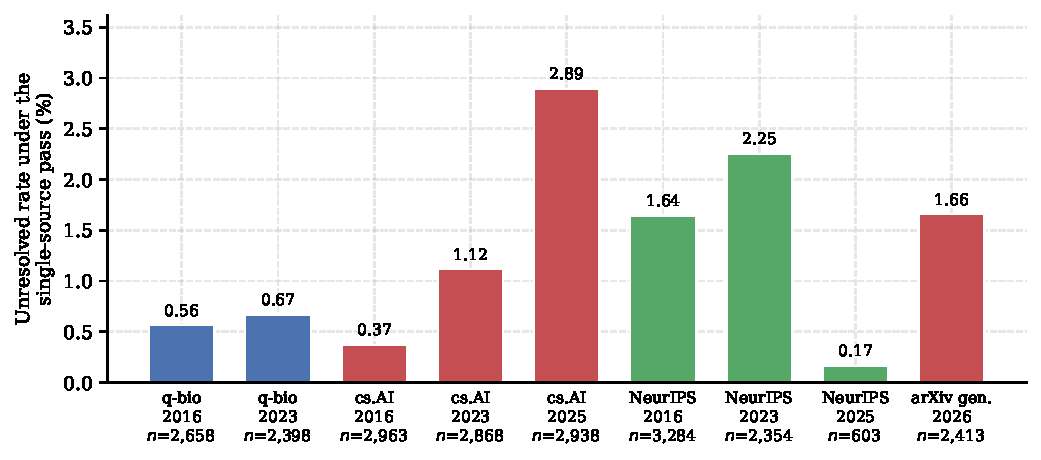
\includegraphics[width=\textwidth]{figures/fig1_unresolved_by_venue.pdf}
\caption{Unresolved rate under the single-source pass, by venue and year. The 2025 NeurIPS estimate rests on \NrefsNipsTwentyfive{} strings and a single unresolved case, and should be read with caution.}
\label{fig:unresolved}
\end{figure}

Applying normalization and multi-source retrieval to those \Nflag{} strings changes the picture substantially. Of the \StageAn{} strings, \StageArecovered{} (\PcStageArecovered{}\%) are recovered outright, in the sense that at least one source returns a record satisfying the full agreement rule, with a DOI or repository identifier recorded as evidence. A further \StageAfuzzy{} (\PcStageAfuzzy{}\%) return partial title agreement and are classified as fuzzy. Only \StageAunresolved{} (\PcStageAunresolved{}\%) remain unmatched across all four sources. The dominant content of the unresolved class is therefore not absent works but strings the screening pass could not match for reasons internal to extraction and retrieval.

Every string in that residual was then resolved individually, and Table~\ref{tab:residual} reports the outcome. Two categories were assigned by rules applied uniformly, namely that a string carrying several distinct years, several DOIs or several \textit{et al.} markers is a block of references the segmenter failed to split, and that a string with no year, no DOI and no author pattern is not a reference. The remaining strings were resolved against a named source, with the identifier or URL recorded so that any verdict can be rechecked without repeating the search.

\begin{table}[htbp]
\centering
\caption{Individual resolution of the \StageBn{} strings that no source matched.}
\label{tab:residual}
\vspace{4pt}
\begin{tabular}{lrrl}
\toprule
\textbf{Category} & \textbf{Strings} & \textbf{Share} & \textbf{Content} \\
\midrule
Segmentation failure & \StageBseg{}    & \PcStageBseg{}\%    & several references concatenated into one string \\
Not a reference      & \StageBnotref{} & \PcStageBnotref{}\% & formulas, tables, prompts, appendix prose \\
Rule limitation      & \StageBrule{}   & \PcStageBrule{}\%   & indexed work the agreement rule could not confirm \\
Coverage limitation  & \StageBcov{}    & \PcStageBcov{}\%    & software, web resources, grey literature \\
Fabrication          & \StageBfab{}    & \PcStageBfab{}\%    & no corresponding work located \\
\bottomrule
\end{tabular}
\end{table}

The residual is thus dominated by two failures of the extraction stage rather than by absent works. The larger, at \StageBseg{} strings, is a segmentation failure with a clear and instructive cause: \StageBastro{} of them come from the 2026 general arXiv cohort and are astronomy bibliographies, where the prevailing A\&A and ApJ styles carry no enumeration marker for the segmenter to key on, so entire reference lists arrive as a single string. This is a property of the encounter between one parser and one citation style, not of the literature, and it accounts for much of what distinguishes the 2026 cohort in Table~\ref{tab:venue}. A further \StageBnotref{} strings are not references at all. The \StageBrule{} strings classed as rule limitations are genuine and indexed works that the agreement rule could not confirm, generally because the string carries no title to compare against, as with a bare DOI, or because the 500-character field limit truncated the entry before its year. Only \StageBcov{} are coverage limitations in the strict sense, namely software releases, web resources and grey literature that none of the four sources indexes, which is where the coverage literature would place them \citep{visser2021, verabaceta2019}.

No string in the residual is a fabrication. One case deserves mention because it illustrates how far an extraction artifact can travel: a reference rendered as an unreadable sequence of symbols, which a single constant character shift restores to Abid, Farooqi and Zou on anti-Muslim bias in language models, the document having embedded a font subset with a custom encoding and no usable character map. The mechanism is real but appears in essentially no other string in the corpus, so it is a curiosity rather than an explanation.

\subsection{The accepted class}
\label{sec:accepted}

The complementary question is whether acceptance by the screening pass establishes anything about the cited work. It does not, at least not to the degree usually assumed. Applying the agreement rule to the record the pass actually accepted, across the full accepted stratum of \Nverified{} references, gives the distribution in Table~\ref{tab:match}. Only \Pcmatchcorrect{}\% of accepted references are matched to a record agreeing with the string on title and year. A further \Pcmatchweak{}\% show partial agreement. The remaining \Nmatchwrong{} references, or \Pcmatchwrong{}\% of the accepted stratum, are matched to a record that does not correspond to the work cited.

\begin{table}[htbp]
\centering
\caption{Agreement between the reference string and the record accepted by the single-source pass, over the full accepted stratum ($n = \Nverified{}$).}
\label{tab:match}
\vspace{4pt}
\begin{tabular}{lrr}
\toprule
\textbf{Outcome of the agreement rule} & \textbf{References} & \textbf{Share} \\
\midrule
Correct match         & \Nmatchcorrect{} & \Pcmatchcorrect{}\% \\
Weak match            & \Nmatchweak{}    & \Pcmatchweak{}\% \\
Wrong record matched  & \Nmatchwrong{}   & \Pcmatchwrong{}\% \\
\bottomrule
\end{tabular}
\end{table}

The failures are not marginal disagreements over formatting. To take three cases from the corpus, a reference to Dai, Olah and Le on document embedding with paragraph vectors was accepted against a 2024 commentary on quantum mechanical statistics; a reference to Yeung and co-authors on over-pruning in variational autoencoders was accepted against a 2025 paper on multi-agent reinforcement learning; and a reference to Babai's chapter in the \textit{Handbook of Combinatorics} was accepted against a 1982 article on Cayley graphs. In each case the cited work exists, the retrieved record exists, and they are different publications. A system reporting these as verified has established nothing about the reference, and an audit scoring only its flagged cases has no way of noticing. The phenomenon is not confined to large corpora processed automatically: in preparing the bibliography of this paper, a single-source query for the OpenAlex description paper returned a different article by overlapping authors on a related topic, which we detected only because the record was inspected by hand.

Two implications follow for the interpretation of unverifiable-citation rates. The denominator of such a rate is not a set of confirmed references, and a fabricated reference would in most cases be accepted rather than flagged, since a permissive matcher returns some record for almost any bibliographic query. Figure~\ref{fig:match} shows that agreement also varies by stratum, with quantitative biology retaining correct-match shares up to \Pcmatchcorrectmax{}\% against \Pcmatchcorrectmin{}\% at the lower end among the computer science strata.

The second implication can be tested directly, and it is the only route by which this design can say anything about fabrication. We drew a stratified random sample of \StageCn{} accepted references, proportional across the nine venue-year strata, and verified each one independently by normalizing the string and querying the four sources under the agreement rule, without reference to the record the screening pass had accepted. Of these, \StageCconfirmed{} (\PcStageCconfirmed{}\%) were confirmed outright against an identifier and \StageCfuzzy{} (\PcStageCfuzzy{}\%) returned partial title agreement. The \StageCunresolved{} that no source confirmed were then resolved individually, with the identifier backing each verdict recorded alongside it. Ten proved to be rule limitations, that is, works indexed and locatable but not confirmable by the rule, generally because a long author list, a concatenated figure caption or a bare URL leaves the rule too little to compare; four were coverage limitations, comprising a research dataset, a news report, an older NIPS proceedings paper and an article in a journal Crossref does not index; and one was not a reference. Two could not be pinned to an exact record, in both cases because related work by the same author group was located but the specific article was not identified.

No fabricated reference was found in the sample. Treating the two unpinned strings as genuine gives an exact upper confidence bound of \Boundfab{}\% on fabrication prevalence in the accepted stratum at the 95\% level; treating both as fabrications, which is the most adverse reading the evidence permits, raises that bound to \Boundconservative{}\%. Neither bound is tight, and the design has no power to estimate a low non-zero prevalence, which is worth stating given that the rates reported by \citet{sakai2026} and \citet{russinovich2026} would predict well under one fabrication in a sample of this size. What the exercise does establish is that the wrong-match rate in Table~\ref{tab:match} does not conceal a reservoir of fabricated references, and that the same pattern found in the flagged class, in which apparent failures resolve into limitations of the rule and of coverage, holds in the accepted class as well.

\begin{figure}[htbp]
\centering
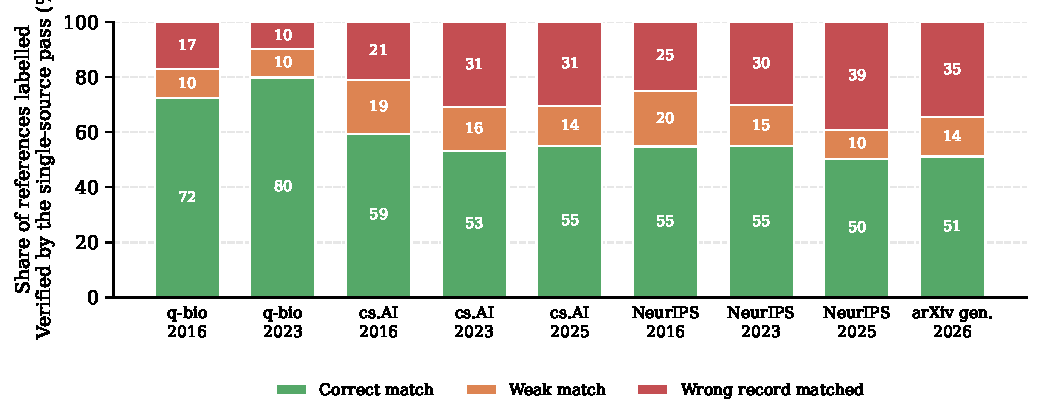
\includegraphics[width=\textwidth]{figures/fig2_verified_match_quality.pdf}
\caption{Agreement between the reference string and the record accepted by the single-source pass, by venue and year.}
\label{fig:match}
\end{figure}

\subsection{Two candidate mechanisms, neither supported}
\label{sec:mechanisms}

Within arXiv Computer Science the unresolved rate rises monotonically, from \FlagrateCsSixteen{}\% in 2016 to \FlagrateCsTwentythree{}\% in 2023 and \FlagrateCsTwentyfive{}\% in 2025 ($\chi^2 = \Cstrendchisq{}$, $\mathrm{df} = \Cstrenddf{}$, $\Cstrendp{}$), so the aggregate trend is not merely a composition effect. In quantitative biology, considerably less exposed to model-assisted writing over the same period, the rate is essentially flat (\FlagrateQbioSixteen{}\% against \FlagrateQbioTwentythree{}\%, Fisher exact $\Qbiop{}$). Within NeurIPS the rate rises between 2016 and 2023 (Fisher exact $\Nipsp{}$) and then falls to \FlagrateNipsTwentyfive{}\% in 2025 on a small subset. It is not easy to construct a behavioural account in which fabricated citations recede at one of the most exposed venues in the same year in which \textit{cs.AI} preprints nearly triple their unresolved rate.

The natural alternative is that the instrument changed rather than the behaviour, since the community shifted progressively from pdfTeX towards XeLaTeX and LuaLaTeX over this period and the resulting differences in how glyphs reach the text stream would degrade extraction unevenly across venues. The corpus does not record compilation metadata, so the engine cannot be identified directly, but it does permit a test of the observable consequence. Table~\ref{tab:damage} counts three signatures of extraction damage in every string: a surviving Unicode ligature, a lost inter-field space, and a line-break hyphen carried into the string. The test does not support the hypothesis.

\begin{table}[htbp]
\centering
\caption{Extraction damage by venue and year, as a percentage of strings. Lost-space counts exclude legitimate camel-case tokens. The final column repeats the unresolved rate for comparison.}
\label{tab:damage}
\vspace{4pt}
\begin{tabular}{lrrr}
\toprule
\textbf{Sub-corpus} & \textbf{Ligature} & \textbf{Lost space} & \textbf{Unresolved} \\
\midrule
arXiv \textit{q-bio} (2016) & \LigQbioSixteen{}\%     & \GlueQbioSixteen{}\%     & \FlagrateQbioSixteen{}\% \\
arXiv \textit{q-bio} (2023) & \LigQbioTwentythree{}\% & \GlueQbioTwentythree{}\% & \FlagrateQbioTwentythree{}\% \\
arXiv \textit{cs.AI} (2016) & \LigCsSixteen{}\%       & \GlueCsSixteen{}\%       & \FlagrateCsSixteen{}\% \\
arXiv \textit{cs.AI} (2023) & \LigCsTwentythree{}\%   & \GlueCsTwentythree{}\%   & \FlagrateCsTwentythree{}\% \\
arXiv \textit{cs.AI} (2025) & \LigCsTwentyfive{}\%    & \GlueCsTwentyfive{}\%    & \FlagrateCsTwentyfive{}\% \\
NeurIPS (2016)              & \LigNipsSixteen{}\%     & \GlueNipsSixteen{}\%     & \FlagrateNipsSixteen{}\% \\
NeurIPS (2023)              & \LigNipsTwentythree{}\% & \GlueNipsTwentythree{}\% & \FlagrateNipsTwentythree{}\% \\
NeurIPS (2025)              & \LigNipsTwentyfive{}\%  & \GlueNipsTwentyfive{}\%  & \FlagrateNipsTwentyfive{}\% \\
arXiv general (2026)        & \LigGenTwentysix{}\%    & \GlueGenTwentysix{}\%    & \FlagrateGenTwentysix{}\% \\
\bottomrule
\end{tabular}
\end{table}

Ligature damage falls sharply over the period, from \LigCsSixteen{}\% to \LigCsTwentyfive{}\% within arXiv \textit{cs.AI} and from \LigNipsSixteen{}\% to \LigNipsTwentyfive{}\% within NeurIPS, so its rank correlation with the unresolved rate across the nine strata is negative ($\rho = \RhoLig{}$). Lost spaces show no relationship ($\rho = \RhoGlue{}$) and the combined indicator correlates negatively ($\rho = \RhoDamage{}$). At the level of the individual string, damage does raise the risk of remaining unresolved by a factor of \Damagerr{}, so the mechanism is real; it is simply not distributed as the temporal trend would require. One methodological point deserves note, since it reverses the apparent result. A naive test for lost spaces, matching a lowercase letter followed directly by an uppercase one, is dominated by legitimate camel-case tokens, above all \textit{arXiv}, whose frequency in these bibliographies roughly quadruples over the period for reasons unrelated to extraction. Before excluding such tokens the lost-space rate appears to rise steeply and to track the unresolved rate; afterwards the apparent trend disappears.

A second candidate fares no better. Citations to preprints and similar material that Crossref indexes poorly become considerably more common, rising within arXiv \textit{cs.AI} from \PreprintshareCsSixteen{}\% of references in 2016 to \PreprintshareCsTwentyfive{}\% in 2025, and such references are more likely to remain unresolved by a factor of \Preprintrr{}. A compositional shift of this size might in principle account for the trend. It does not, because the trend is present within each category taken separately: among references mentioning no preprint server at all, the unresolved rate in arXiv \textit{cs.AI} still rises from \NonpreprintrateCsSixteen{}\% to \NonpreprintrateCsTwentythree{}\% and \NonpreprintrateCsTwentyfive{}\%.

We therefore do not identify the mechanism behind the temporal trend, and we would rather say so than offer an account the data do not carry. What the analysis establishes is narrower but sufficient for the argument. Whatever drives the rise, it drives a rise in retrieval failures on works that exist, since \PcStageArecovered{}\% of the unresolved strings are recovered once retrieval is done properly. The trend is therefore not evidence about citation behaviour, whatever ultimately explains it.

\section{Discussion and conclusions}
\label{sec:disc}

This paper has treated automated reference verification as a measurement problem and examined both of its output classes on a corpus of \Nrefs{} reference strings from \Npapers{} papers published between 2016 and 2026. The unresolved class is dominated by recoverable retrieval failures, so that a naive unresolved rate overstates any quantity of substantive interest by a wide and time-varying margin. The accepted class is also unreliable, with \Pcmatchwrong{}\% of accepted references resolving to a publication other than the one cited, a failure mode invisible to evaluations that score only flagged cases.

For those operating screening systems the two error modes have different costs and call for different remedies. False alarms on genuine references are expensive because each consumes editorial time and may raise an unwarranted question about a manuscript, and they are reduced substantially by normalization and by querying more than one source. False confirmations are cheaper per case but more corrosive, because they accumulate silently and leave the output uninformative in the direction that matters most. The remedy there is not more sources but a comparison step, since accepting the top-ranked record without checking title, author and year agreement produces a wrong record roughly a quarter of the time on this corpus. Given that arXiv now suspends authors on the basis of unchecked references \citep{naturebanned2026}, the asymmetry between a system that flags too much and one that confirms too readily deserves more attention than it has received.

For researchers measuring citation hallucination in the record, we would offer the decomposition as a calibration rather than as a rebuttal. The phenomenon documented by \citet{sakai2026}, \citet{zhao2026} and \citet{russinovich2026} is real and nothing here suggests otherwise. The point is narrower: an unresolved rate computed from a single-source matcher on unnormalized strings contains a large and time-varying component unrelated to authorship, and the direction of the bias is not constant across fields or years. The design of \citet{russinovich2026} already responds to that problem, and their reported reference-level rates below one per cent are consistent with a large share of naive flags being artifacts. Our results suggest the second problem, the permissiveness of the accept decision, deserves symmetric treatment, since a study validating only its flagged cases cannot bound what its accepted cases contain.

For those constructing bibliometric indicators the implication is that raw unverifiable-citation rates should not be used as measures of research integrity. A large component of such a rate reflects database coverage and extraction fidelity, neither of which is a property of the citing author, and both of which vary across fields and over time. An indicator omitting the decomposition will track changes in tooling and indexing while appearing to track changes in behaviour.

Several limitations qualify these conclusions, and the first is scope. The corpus covers computer science, quantitative biology and one general cohort, in texts almost entirely in English, and the balance between the error modes will differ wherever metadata coverage is weaker, particularly in the humanities, in law and in non-English publication \citep{verabaceta2019}. The proportions reported here are properties of this corpus and this extraction pipeline rather than constants of the literature.

The extraction pipeline is a second limitation, and a consequential one. Segmentation is heuristic rather than model-based, which admits non-reference material into the corpus, and the fifty-reference cap truncates \Ntruncated{} of the \Npapers{} bibliographies. A model-based parser such as GROBID \citep{lopez2009} or CERMINE \citep{tkaczyk2015} would segment more accurately, and replicating the analysis under such a parser would establish how much of the unresolved class is attributable to segmentation rather than to the text layer. We would expect the qualitative conclusion to survive, since the wrong-match result does not depend on segmentation quality, but this has not been shown. Third, the comparison in Table~\ref{tab:benchmark} is against a deliberately simple screening pass rather than a deployed system, and a head-to-head evaluation against the architecture of \citet{russinovich2026} on a common subset would be a considerably more demanding test.

A fourth limitation concerns the provenance of the audit itself, and we would rather be explicit about it than let a reader assume otherwise. The verification reported in Sections~\ref{sec:unresolved} and \ref{sec:accepted} was carried out by an automated agent with programmatic access to the four sources and to web search, and not by a human expert coder. Every verdict is backed by a recorded identifier or URL and each rule-based category is reproducible from the released scripts, which is a stronger evidentiary standard than a manual audit usually offers. It is nonetheless a single automated coder, so no inter-rater reliability statistic is available, and the coding sheets released with the data reserve a quarter of the strings in each set for an independent second coder should one become available. The boundary between a work that no index covers and a work that does not exist is the judgement most exposed to this limitation, which is why the identifier behind every such verdict is recorded individually rather than summarised.

Finally, and most plainly, we do not explain the temporal trend. Both mechanisms we were able to test fail to account for it, and identifying it would require compilation metadata the corpus does not carry and probably a source-level rather than a PDF-level corpus. The fabrication bounds reported in Section~\ref{sec:accepted} are correspondingly loose, and this design has no power to estimate a low non-zero prevalence. We prefer to state that position plainly rather than to report a precision the evidence does not support.

\section*{CRediT author contribution statement}
\textbf{Diletta Abbonato:} Conceptualization, Methodology, Software, Formal analysis, Data curation, Writing (original draft), Writing (review and editing).

\section*{Data availability statement}
The corpus ($N = \Nrefs{}$ reference strings) and the evaluation data are openly available at \url{https://github.com/zabbonat/References-Validation}.

\section*{Code availability statement}
The verification engine, the analysis scripts and the code generating every quantity reported in this manuscript are released under an MIT licence at \url{https://github.com/zabbonat/References-Validation}.

\section*{Conflicts of interest}
The author develops and maintains the CheckIfExist software evaluated in this study, and implemented the single-source screening pass against which it is compared. The author declares no competing financial interests.

\section*{Ethics statement}
This analysis evaluates published academic literature and involves no human or animal subjects.

\bibliographystyle{apalike}
\bibliography{references}

\end{document}
